\documentclass[oneside]{amsart}

\usepackage[all]{xy}
\usepackage{tikz-cd}
\usepackage[T1]{fontenc}
\usepackage{xstring}
\usepackage{xparse}
\usepackage{xr-hyper}
\usepackage{xcolor}
\definecolor{brightmaroon}{rgb}{0.76, 0.13, 0.28}
\usepackage[linktocpage=true,colorlinks=true,hyperindex,citecolor=blue,linkcolor=brightmaroon]{hyperref}
\usepackage[nameinlink]{cleveref}
\usepackage[left=1.25in,right=1.25in,top=0.75in,bottom=0.75in]{geometry}
%\usepackage[charter,greekfamily=didot]{mathdesign}
%\usepackage{Baskervaldx}
\usepackage{amssymb}
\usepackage{stmaryrd}
\usepackage{mathrsfs}
\usepackage{mathpazo}
\linespread{1.05}

\usepackage[nobottomtitles]{titlesec}
\usepackage{marginnote}
\usepackage{enumerate}
\usepackage{longtable}
\usepackage{aurical}
\usepackage{microtype}

\newtheoremstyle{ega-env-style}%
{}{}{\rmfamily}{}{\bfseries}{.}{ }{\thmnote{(#3)}}%

\newtheoremstyle{ega-thm-env-style}%
{}{}{\itshape}{}{\bfseries}{. --- }{ }{\thmname{#1}\thmnumber{ #2}\thmnote{ (#3)}}%

\newtheoremstyle{ega-defn-env-style}%
{}{}{\rmfamily}{}{\bfseries}{. --- }{ }{\thmname{#1}\thmnumber{ #2}\thmnote{ (#3)}}%

\theoremstyle{ega-env-style}
\newtheorem*{env}{---}

\theoremstyle{ega-thm-env-style}
\newtheorem{theorem}{Theorem}[subsection]
\newtheorem{proposition}{Proposition}[subsection]
\newtheorem{lemma}{Lemma}[subsection]
\newtheorem{corollary}{Corollary}[subsection]
\newtheorem{stheorem}{Theorem}[section]
\newtheorem{slemma}[stheorem]{Lemma}
\newtheorem{skey}[stheorem]{Key Formula}
\newtheorem{conjecture}{Conjecture}[subsection]

\theoremstyle{ega-defn-env-style}
\newtheorem*{definition}{Definition}
\newtheorem{example}{Example}[subsection]
\newtheorem*{examples}{Examples}
\newtheorem*{remark}{Remark}
\newtheorem*{remarks}{Remarks}
\newtheorem*{notation}{Notation}
\newtheorem*{exercise}{Exercise}
\newtheorem*{properties}{Properties}
\newtheorem*{consequences}{Consequences}
\newtheorem*{note}{Note}
\newtheorem*{fact}{Fact}

\makeatletter
\def\l@subsection{\@tocline{2}{0pt}{2.5pc}{2.2pc}{}}
\def
\section{\@startsection{section}{1}%
	\z@{.7\linespacing\@plus\linespacing}{.5\linespacing}%
{\normalfont\bfseries\Large\scshape\centering}}
\renewcommand{\@seccntformat}[1]{%
	\ifnum\pdfstrcmp{#1}{section}=0\textsection\fi%
\csname the#1\endcsname.~}
\makeatother

\def\mathcal{\mathscr}
%% Fonts

\def\sh{\mathcal}                   % sheaf font
\def\bb{\mathbf}                    % bold font
\def\cat{\mathsf}                   % category font

%% Font Letters

\def\CL{\mathcal{L}}
\def\OO{\mathcal{O}}
\def\CX{\mathcal{X}}

%% Cohomology

\def\CH{\mathrm{H}}                 % cohomology H
\def\CHH{\check{\HH}}               % Čech cohomology H
\def\RD{\mathrm{R}}                 % right derived R
\def\LD{\mathrm{L}}                 % left derived L
\def\dual#1{{#1}^\vee}              % dual
\def\Tor{\operatorname{Tor}}        % Tor
\def\Ext{\operatorname{Ext}}        % Ext
\def\HdR{\mathrm{H}_{\mathrm{dR}}}  % de Rham cohomology
\def\Zc{\underline{\mathbb{Z}}}     % constant sheaf with integer coeffs

%% Categories

\def\A{\cat{A}}                     % category A, usually abelian
\def\C{\cat{C}}                     % category C
\def\op{^\cat{op}}                  % opposite category
\def\Set{\cat{Sets}}                % category of sets
\def\Grp{\cat{Gps}}                 % category of groups
\def\Alg{\cat{Alg}}                 % category of algebras
\def\QCoh{\cat{QCoh}}               % category of quasicoherent sheaves
\def\supertilde{{\,\widetilde{\,}\,}}   % use \supertilde instead of ^\sim
\def\Hom{\operatorname{Hom}}        % morphisms
\def\End{\operatorname{End}}        % endomorphisms
\def\Aut{\operatorname{Aut}}        % automorphisms
\def\ker{\operatorname{ker}}        % kernel
\def\img{\operatorname{im}}         % image
\def\coker{\operatorname{coker}}    % cokernel
\def\pr{\operatorname{pr}}          % projection
\def\EssIm{\operatorname{EssIm}}    % essential image
\DeclareMathOperator*{\colim}{colim}   % colimit


%% Schemes

\def\Proj{\operatorname{Proj}}      % Proj
\def\Supp{\operatorname{Supp}}      % support
\def\Spec{\operatorname{Spec}}      % Spec
\def\Spf{\operatorname{Spf}}        % formal Spec
\def\Aff{\mathbb A}                 % affine space
\def\P{\mathbb{P}}                  % projective space
\def\Pic{\operatorname{Pic}}        % Picard group

%% Standard Operators

\def\codim{\operatorname{codim}}    % codimension
\def\id{\operatorname{id}}          % identity

%% Arrows
\renewcommand{\to}{\mathchoice{\longrightarrow}{\rightarrow}{\rightarrow}{\rightarrow}}
\newcommand{\from}{\mathchoice{\longleftarrow}{\leftarrow}{\leftarrow}{\leftarrow}}
\let\mapstoo\mapsto
\renewcommand{\mapsto}{\mathchoice{\longmapsto}{\mapstoo}{\mapstoo}{\mapstoo}}
\def\isoto{\simeq}                  % isomorphism
\def\simto{\xrightarrow{\sim}}      % isomorphism arrow
\def\surjto{\twoheadrightarrow}     % surjetion
\def\injto{\hookrightarrow}         % injection

%% Under/Over Accents

\newcommand{\wh}[1]{\widehat{#1}}   % hat
\newcommand{\wt}[1]{\widetilde{#1}}    % tilde
\def\ul{\underline}                % underline

%% Spaces

\def\Z{\mathbb Z}                  % integers
\def\Q{\mathbb Q}                  % rationals
\def\N{\mathbb{N}}                 % naturals

%% Groups

\def\GL{\bb{GL}}                   % general linear group
\def\SL{\bb{SL}}                   % special linear group
\def\det{\operatorname{det}}       % determinant

%% Sub/Superscripts

\def\et{^\text{\'et}}              % \'etale
\def\an{^{\text{an}}}              % analytic

%% Misc

\newcommand{\defn}[1]{\textbf{#1}}  % definition highlighting
\def\defeq{:=}                     % definition equation
\def\eps{\varepsilon}              % correct epsilon
\newcommand{\gen}[1]{\left\langle\!\left\langle #1 \right\rangle\!\right\rangle}



\def\shHom{\sh{H}\textup{\kern-2.2pt{\Fontauri\slshape om}}}   % sheaf Hom
\def\shProj{\sh{P}\textup{\kern-2.2pt{\Fontauri\slshape roj}}} % sheaf Proj
\def\shExt{\sh{E}\textup{\kern-2.2pt{\Fontauri\slshape xt}}}   % sheaf Ext
\def\shGr{\sh{G}\textup{\kern-2.2pt{\Fontauri\slshape r}}}     % sheaf Gr
\def\shDer{\sh{D}\,\textup{\kern-2.2pt{\Fontauri\slshape er}}} % sheaf Der
\def\shDiff{\sh{D}\,\textup{\kern-2.2pt{\Fontauri\slshape if{}f}}\,} % sheaf Diff
\def\shHomcont{\sh{H}\textup{\kern-2.2pt{\Fontauri\slshape om.\,cont}}}   % sheaf Hom.cont
\def\shAut{\sh{A}\textup{\kern-2.2pt{\Fontauri\slshape ut}}}   % sheaf Aut
\def\shSym{\sh{S}\textup{\kern-2.2pt{\Fontauri\slshape ym}}}   % sheaf Sym

\makeatletter
\newcommand{\cbigoplus}{\DOTSB\cbigoplus@\slimits@}
\newcommand{\cbigoplus@}{\mathop{\widehat{\bigoplus}}}
\makeatother


\def\CC{\mathcal C}
\def\CS{\mathcal S}
\def\CT{\mathcal T}
\def\Sing{\operatorname{Sing}}
\def\map{\operatorname{map}}
\def\Mor{\operatorname{Mor}}
\def\1b{\mathbb{1}}
\def\R{\bb{R}}
\def\Ch{\cat{Ch}}
\def\Cone{\operatorname{Cone}}
\def\S{\mathbb{S}}
\def\smap{\operatorname{smap}}

\title{Infinity Categories}
\author{Lecturer: Pramod Achar,\quad Typesetter: Micha{\l} Mruga{\l}a}

\begin{document}

\begin{center}
	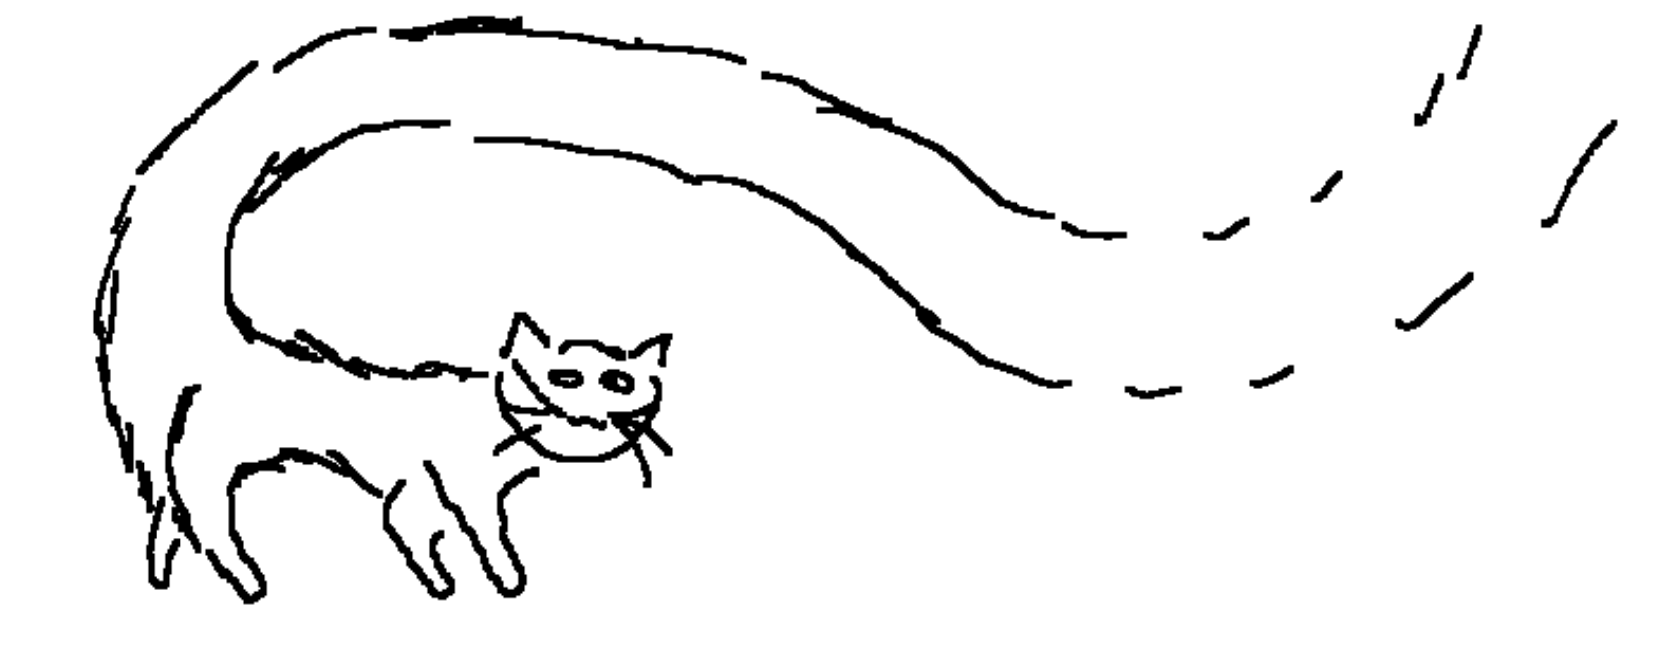
\includegraphics[width=0.5\textwidth]{TheInfinityCat.png}
	\footnote{Artwork by Leonardo Colombo.}
\end{center}
\maketitle

\section{Simplicial sets}

\begin{definition}
	The \defn{simplex category} $\bb{\Delta}$ is the category of
	\begin{itemize}
		\item finite non-empty totally ordered sets
		\item order-preserving maps.
	\end{itemize}
\end{definition}
\begin{notation}
	$[n]=\{0<1<2<\dots<n\} $ for $n\in \Z_{\ge 0}$.
\end{notation}
Every object in $\bb{\Delta}$ is (uniquely) isomorphic to some $[n]$.
\begin{definition}
	A \defn{simplicial set} is a functor
	\[
		\CS:\bb{\Delta}\op \to \Set
	\]
\end{definition}
\begin{notation}
	$\CS_n \defeq \CS([n])$, call this the \defn{set of $n$-simplices} of $\CS$. 0-simplices
	are called \defn{vertices}, 1-simplices are called \defn{edges}.
\end{notation}
\begin{example}
	Let $C$ be a set. Let $\ul{C}:\bb{\Delta}\op\to \Set$ be the constant functor:
	\begin{gather*}
		\ul{C}_n = C\quad \forall n, \\
		\ul{C}(\alpha) = \id \quad \forall \alpha:[m]\to [n] \text{ in }\bb{\Delta}.
	\end{gather*}
	This is called a \defn{discrete simplicial set}.
\end{example}
\begin{definition}
	Let $\CS$ be a simplicial set. Given $\alpha:[n]\to [n-1]$ we get
	$\CS(\alpha):\CS_{n-1}\to \CS_n$. The $n$-simplices in the image are called
	\defn{degenerate} simplices, i.e. $\sigma$ is degenerate if there is an $\alpha$ such
	that $\sigma\in \img(\CS(\alpha))$.
\end{definition}
\begin{lemma}
	A simplicial set is discrete if and only if for all $n\ge 1$ all $n$-simplices are degenerate.
\end{lemma}
\begin{exercise}
	Prove it.
\end{exercise}
\begin{example}
	Let $(P,\ge )$ be a poset. Define a simplicial set $N(P,\le )$ called the \defn{nerve}
	of $(P,\le )$ by
	\[
		N(P,\le )_k = \{\text{chains }p_0\le p_1\le \dots\le p_k: p_i\in P\}
	\]
	where a chain is a totally ordered subset.
\end{example}
\begin{exercise}
	Finish the definition. Which simplices are degenerate?
\end{exercise}
\begin{example}[``Standard $n$-simplex'']
	The \defn{standard $n$-simplex} is
	\[
		\Delta^{n} \defeq N([n]).
	\]
	(Pictures)
\end{example}
\begin{note}
	For $j\in [n]$, we get a subsimplicial set
	\[
		N([n]\setminus \{j\} ) \subset \Delta^{n}
	\]
	isomorphic to $\Delta^{n-1}$ called the $j\th$ \defn{face} of $\Delta^{n}$. (Picture)
\end{note}
\begin{example}[Horns]
	Let $n\ge 0$ and $0\le j\le n$, define the \defn{horn}
	\[
		\Lambda^{n}_j \defeq
		\begin{array}{c}
			\text{subsimplicial set of }\Delta^{n} = N([n]) \\
			\text{consisting of chains }p_0\le p_1\le \dots\le p_k \\
			\text{such that } \{p_0,\dots,p_k\} \not\supset [n] \setminus \{j\} .
		\end{array}
		(Pictures)
	\]
\end{example}
\begin{example}[$(n-1)$-sphere $\partial\Delta^{n}$]
	We define the \defn{$(n-1)$-sphere}
	\[
		\partial \Delta^{n} \defeq
		\begin{array}{c}
			\text{subsimplicial set of }\Delta^{n} \\
			\text{chains }p_0\le \dots \le p_k\text{ such that }\{p_0\le \dots\le p_k\} \neq [n]
		\end{array}
	\]
\end{example}
\begin{example}[Products]
	Let $\CS,\CT$ be simplicial sets. We define their \defn{product} $\CS\times \CT$ as
	\[
		(\CS\times \CT)_k = \CS_k \times \CT_k.
	\]
	(Picture)
\end{example}
\begin{example}
	Let $\C$ be an ordinary category. We define its \defn{nerve} $N(\C)$ as
	\[
		N(\C)_k \defeq \left\{
			\begin{array}{c}
				\text{composable sequences of morphisms} \\
				X_0 \xrightarrow{f_1} X_1\xrightarrow{f_2}X_2\to \dots\xrightarrow{f_k} X_k
		\end{array}\right\} .
	\]
\end{example}
\begin{example}
	Let $X$ be a topological space. The \defn{singular simplicial set} of $X$ is defined as
	\[
		\Sing(X)_k = \{\text{continuous maps }|\Delta^{k}|\to X\} ,
	\]
	where $|\Delta^{k}|$ is the standard $k$-simplex
	\[
		|\Delta^{k}| = \left\{ (x_0,\dots,x_k)\in \bb{R}^{k+1} \middle| x_i\ge 0, \sum x_i=1 \right\} .
	\]
\end{example}
\begin{exercise}
	What does this do to the morphisms in $\bb{\Delta}$?
\end{exercise}
\begin{definition}
	A \defn{Kan complex} is a simplicial set $X$ such that for every diagram
	\[
		\begin{tikzcd}
			\Lambda^{n}_j \ar[r,"\text{any map}"] \ar[d,hook] & X \\
			\Delta^{n} \ar[ur,dashed]
		\end{tikzcd}
	\]
	we can fill the dashed arrow. This is called an \defn{extension problem}. If the arrow
	exists we say that the extension problem \defn{admits a solution}.
\end{definition}
Daniel Kan discovered Kan complexes in 1958. The \emph{key fact} is that $\Sing(X)$
\emph{is} a Kan complex. The theme from 1958 to today is that Kan complexes are a
``combinatorial model'' for algebraic topology which allows us to do homotopy theory.

\begin{definition}
	Let $X$ be a Kan complex and $\CS$ be any simplicial set. Two maps $f,g:\CS\to X$ are
	said to be \defn{homotopic} if there exists a map $H:\CS\times \Delta^{1}\to X$ such that
	\[
		H|_{\CS\times \{0\} } = f,\quad H|_{\CS\times \{1\} } = g.
	\]
\end{definition}
\begin{lemma}
	This is an equivalence relation.
\end{lemma}
\begin{proof}
	Omitted, tricky for an exercise. This requires $X$ to be a Kan complex.
\end{proof}
\begin{definition}
	Let $X$ be a Kan complex and $x_0$ be a vertex of $X$. Let
	\[
		\text{Loops}_{x_0} = \{\text{maps }\gamma:\Delta^{n}\to X\text{ such that
		}\gamma|_{\partial\Delta^{n}}\text{ is the constant map to }x_0\}.
	\]
	We say $\gamma,\gamma'\in \text{Loops}_{x_0}$ are \defn{relatively homotopic}
	(\defn{rel. homotopic}) if there exists $H:\Delta^{n}\times \Delta^{1}\to X$ such that
	\[
		H|_{\Delta^{n}\times \{0\} } = \gamma,\quad H|_{\Delta^{n}\times \{1\} } =
		\gamma',\quad H|_{\partial \Delta^{n}\times \Delta^{1}} = \text{const. map to }x_0.
	\]
	Define
	\[
		\pi_n(X,x_0) \defeq \frac{\text{Loops}_{x_0}}{\text{rel. homotopy}}.
	\]
\end{definition}
\begin{fact}
	For $n\ge 1$, $\pi_n(X,x_0)$ is a group. For $n\ge 2$, $\pi_n(X,x_0)$ is abelian.
\end{fact}
\begin{definition}
	An \defn{$\infty$-category} (or \defn{quasi-category}) is a simplicial set $\CC$ such
	that any extension problem
	\[
		\begin{tikzcd}
			\Lambda_{j}^{n} \ar[r] \ar[d,hook] & \CC \\
			\Delta^{n} \ar[ur, dashed]
		\end{tikzcd}
	\]
	with $0<j<n$ (\defn{inner horns}) admits a solution. (Picture) An $\infty$-category is
	also called a \defn{weak Kan complex}.
\end{definition}
\begin{lemma}
	Let $\C$ be an ordinary category, then $N(\C)$ is an $\infty$-category.
\end{lemma}
\emph{Digression:} Let $I^{n}$ be the simplicial set consisting of $n$ consecutive
1-simplices (\defn{$n$-spine}) (Picture). A naive alternative definition is: $\CC$ is an
infinity category if every
\[
	\begin{tikzcd}
		I^{n} \ar[r] \ar[d,hook] & \CC \\
		\Delta^{n} \ar[ur]
	\end{tikzcd}
\]
has a solution. This is WRONG (but its wrongness is subtle), even though $N(\text{ord.
cat.})$ satisfy this. There is a book by Markus Land ``Introduction to
$\infty$-categories'' which explores this. The definition of $\infty$-categories was
introduced by Boardman-Vogt in 1972. Joyal started generalizing results from ordinary
category theory to $\infty$-categories in 2006. Lurie is largely responsible for how well
this notion is developed in modern literature.

\begin{remark}
	Having a unique solution to the lifting problem characterizes nerves of ordinary categories.
\end{remark}
\begin{definition}
	Let $\CC$ be an $\infty$-category. An \defn{object} is a vertex. A \defn{morphism} is an
	edge. An \defn{identity morphism} is a degenerate edge. Say that $h$ is \emph{a}
	\defn{composition} of $g$ and $f$ if there exists a 2-simplex such that (Picture).
\end{definition}
\begin{remark}
	Compositions are NOT unique in $\infty$-categories.
\end{remark}
\begin{example}[$\infty$-categories] \leavevmode
\begin{enumerate}[1)]
	\item Topological spaces $\cat{Top}$.
		\begin{itemize}
			\item Objects are topological spaces.
			\item Morphisms are continuous maps.
			\item A 2-simplex is a (not necessarily commutative) diagram
				\[
					\begin{tikzcd}
						& X_1 \ar[dr,"g"] \\
						X_0 \ar[ur,"f"] \ar[rr,"h"] & & X_2
					\end{tikzcd}
				\]
				\emph{and} a homotopy $H:X_0\times [0,1]\to X_2$ from $gf$ to $h$.
			\item A 3-simplex is a diagram
				\[
					\begin{tikzcd}
						& X_0 \ar[dl] \ar[dr] \ar[dd] \\
						X_1 \ar[rr] \ar[dr] & & X_3 \\
						& X_2 \ar[ur]
					\end{tikzcd}
				\]
				with continuous maps $f_{ij}:X_i\to X_j$ for $i<j$, homotopies $T_{ijk}X_i\times
				[0,1]\to X_k$ from $f_{jk}\circ f_{ij}$ to $f_{ik}$, and $H:X_0\times [0,1]^2\to X_3$
				(\defn{higher homotopy}) such that $H|_{\text{bdry}}$ is
				\[
					\begin{tikzcd}
						(0,0) \ar[r,"T_{123}f_{01}"] \ar[d,"f_{23}T_{012}"'] & (0,1) \ar[d,"T_{013}"] \\
						(1,0) \ar[r,"T_{023}"'] & (1,0)
					\end{tikzcd}
				\]
		\end{itemize}
	\item The $\infty$-category of ordinary categories $\cat{Cat}_1$.
		\begin{itemize}
			\item Objects are ordinary categories.
			\item Morphisms are functors.
			\item A 2-simplex is a (not necessarily commutative) diagram
				\[
					\begin{tikzcd}
						& X_1 \ar[dr,"g"] \\
						X_0 \ar[ur,"f"] \ar[rr,"h"] & & X_2
					\end{tikzcd}
				\]
				\emph{and} a natural isomorphism $T:g\circ f \simto h$.
			\item A 3-simplex is a diagram
				\[
					\begin{tikzcd}
						& X_0 \ar[dl] \ar[dr] \ar[dd] \\
						X_1 \ar[rr] \ar[dr] & & X_3 \\
						& X_2 \ar[ur]
					\end{tikzcd}
				\]
				where $f_{ij}$ are functors and $T_{ijk}$ are natural isomorphism such that
				\[
					\begin{tikzcd}
						\bullet \ar[r,"T_{123}f_{01}"] \ar[d,"f_{23}T_{012}"'] & \bullet \ar[d,"T_{013}"] \\
						\bullet \ar[r,"T_{023}"'] & \bullet
					\end{tikzcd}
				\]
				commutes
		\end{itemize}
\end{enumerate}
\end{example}
A source of $\infty$-categories are
\begin{itemize}
\item ordinary categories with an equivalence relation on morphisms,
\item ordinary categories with inverting some morphisms.
\end{itemize}
\marginpar{Lecture 2}
\begin{definition} \leavevmode
\begin{enumerate}[1.]
	\item Let $\C$ be an $\infty$-category and $f:X\to Y$ be a morphism in $\C$. $f$ is
		called an \defn{isomorphism} if there exists $g:Y\to X$ and two 2-simplices
		\[
			\begin{tikzcd}
			 & Y \ar[dr,"g"] & & & X \ar[dr,"f"] \\
				X \ar[ur,"f"] \ar[rr,"\id_X"] & & X & Y \ar[ur,"g"] \ar[rr,"\id_Y"] & & Y
			\end{tikzcd}
		\]
	\item An $\infty$-category is called an \defn{$\infty$-groupoid} if \emph{every}
		morphism is an isomorphism.
\end{enumerate}
\end{definition}
\begin{theorem}[Joyal]
An $\infty$-category is an $\infty$-groupoid if and only if it is a Kan complex.
\end{theorem}
\begin{proof}
The forward direction is hard, the converse is an exercise.
\end{proof}
\begin{definition}\leavevmode
\begin{enumerate}[1.]
		\setcounter{enumi}{2}
	\item Say $f,g:\C\to \cat{D}$ are functors (morphisms of simiplicial sets) of
		$\infty$-categories. A \defn{natural transformation} from $f$ to $g$ is a functor
		$T:\C\times \Delta^{1}\to \cat{D}$ such that $T|_{\C\times \{0\} }=f$ and $T|_{\C\times \{1\}}=g$.

		A special case: the identity natural transformation $\id_f:f\to F$ is the map
		\[
			\begin{tikzcd}
				\C\times \Delta^{1} \ar[r,"\text{proj}"] & \C \ar[r,"f"] & \cat{D}.
			\end{tikzcd}
		\]

		$T:f\to g$ is a \defn{natural isomorphism} if there exists $T':g\to f$ and two maps
		$H:\C\times \Delta^2\to \cat{D},H':\C\times \Delta^2\to \cat{D}$ such that
		\[
			\begin{tikzcd}
				& g \ar[dr,"T'"] & & & f \ar[dr,"T"] \\
				f \ar[ur,"T"] \ar[rr,"\id_f"] & & f & g \ar[ur,"T'"] \ar[rr,"\id_g"] & & g
			\end{tikzcd}
		\]
\end{enumerate}
\end{definition}
In ordinary category theory a natural transformation assigns objects in $\C$ to morphisms
in $\cat{D}$ and morphisms in $\C$ to commutative squares in $\cat{D}$. For
$\infty$-categories a natural transformation takes objects to morphisms, morphisms to
diagrams of shape $\Delta^{1}\times \Delta^{1}$ and generally an $n$-simplex to a diagram
of shape $\Delta^{n}\times \Delta^{1}$.

\begin{theorem}[Pointwise criterion for natural isomorphism]
Let $f,g:\C\to \cat{D}$ be functors of $\infty$-categories and $T:f\to g$ be a natural
transformation. $T$ is a natural isomorphism if and only if for all objects $x$ in $\C$,
$T(\{x\}\times \Delta^{1})$ is an isomorphism in $\cat{D}$.
\end{theorem}
This is a consequence of Joyal's theorem.
\begin{definition}
Define $\cat{Cat}_\infty$ as follows:
\begin{itemize}
	\item Objects are $\infty$-categories.
	\item Morphisms are functors.
	\item 2-simplices are diagrams
		\[
			\begin{tikzcd}
				& X_1 \ar[dr,"g"] \\
				X_0 \ar[ur,"f"] \ar[rr,"h"] & & X_2
			\end{tikzcd}
		\]
		and a natural isomorphism $T:g\circ f\simto h$.
	\item 3-simplices and higher: copy the data of $\cat{Top}$ and replace $[0,1]^{n}$ by
		$(\Delta^{1})^{n}$.
\end{itemize}
\end{definition}
This is similar to $\cat{Top}$ and $\cat{Cat}_1$.
\begin{definition}
Define $\cat{Spc}$ same as above, except objects are $\infty$-groupoids.
\end{definition}
In literature: $\infty$-groupoids, Kan complexes, spaces and anima are synonyms.
\begin{definition}
A functor $f:\C\to \cat{D}$ is called a \defn{categorical equivalence} if there exists
$g:\cat{D}\to \C$ such that $f\circ g\isoto \id_{\cat{D}}$ and $g\circ f\isoto \id_{\C}$.
\end{definition}
\begin{theorem}[Fundamental Theorem of Category Theory]
A functor $f:\C\to \cat{D}$ is a categorical equivalence if and only it it's essentially
surjective and fully faithful.
\end{theorem}
Note that we haven't defined essentially surjective or fully faithful. Let's pre-warm up
first before we define them.

\begin{lemma}
Let $X$ be a Kan complex. $X$ is \defn{contractible} (i.e., categorically equivalent to
$\Delta^{0}$) if and only if every lifting problem
\[
	\begin{tikzcd}
		\partial \Delta^{n} \ar[r] \ar[d] & X \ar[d] \\
		\Delta^{n} \ar[ur,dashed] \ar[r] & \Delta^{0}
	\end{tikzcd}
\]
admits a solution.
\end{lemma}
Now we're warm enough to warm up, so lets do that. Let $f:X\to Y$ be a map of Kan
complexes. Suppose every lifting problem
\[
\begin{tikzcd}
	\partial \Delta^{n} \ar[r] \ar[r] & X \ar[d,"f"] \\
	\Delta^{n} \ar[ur,dashed] \ar[r] & Y
\end{tikzcd}
\]
has a solution. Then $f$ \emph{is} a categorical equivalence (think: homotopy equivalence
of topological spaces). But this condition is too strong for the converse. A simple
counter-example is to take $X$ contractible.

\begin{definition}
Let $f:\C\to \cat{D}$ be a functor of $\infty$-categories. Given
\begin{equation}\label{eq:star}
	\begin{tikzcd}
		\partial \Delta^{n} \ar[r,"r"] \ar[d] & \C \ar[d,"f"] \\
		\Delta^{n} \ar[r,"s"] & \cat{D}
	\end{tikzcd}
\end{equation}
we say it admits a \defn{solution up to isomorphism} if
\begin{enumerate}[(i)]
	\item there exists $u:\Delta^{n}\to \C$ such that
		\[
			\begin{tikzcd}
				\partial \Delta^{n} \ar[r,"r"] \ar[d] & \C \\
				\Delta^{n} \ar[ur,"u"]
			\end{tikzcd}
		\]
	\item $f\circ u:\Delta^{n}\to \cat{D}$ is naturally isomorphic to $s:\Delta^{n}\to
		\cat{D}$ \emph{relative} (of relative homotopy) to $\partial \Delta^{n}$.
\end{enumerate}
\end{definition}
\begin{definition}
Let $f:\C\to \cat{D}$ be a functor of $\infty$-categories.
\begin{itemize}
	\item It's \defn{essentially surjective} if every diagram \eqref{eq:star} with $n=0$
		admits a solution up to isomorphism.
	\item It's \defn{full} if every diagram \eqref{eq:star} with $n=1$ admits a solution up
		to isomorphism.
	\item It's \defn{fully faithful} if every diagram \eqref{eq:star} with $n\ge 1$ admits a
		solution up to isomorphism.
\end{itemize}
\end{definition}
So a functor of $\infty$-categories is fully faithfull and essentially surjective if all
\eqref{eq:star} admit a solution up to isomorphism.
\begin{remark}
These definitions of fully and full faithful are \emph{nonstandard}.
\end{remark}
Now the Fundamental Theorem makes sense.
\begin{proof}[Proof idea]
The forward direction is easy. Conversely, we factor through
\[
	\begin{tikzcd}
		\C \ar[r] & \C^{\text{enhanced}} \ar[r] & \cat{D}
	\end{tikzcd}
\]
where an $n$-simplex in $\C^{\text{enhanced}}$ is the data of
\begin{itemize}
	\item $n$-simplex in $\C$,
	\item a diagram of shape $\Delta^{n}\times \Delta^{1}$ in $\cat{D}$ satisfying some conditions.
\end{itemize}
The inverses of the intermediate maps are easy to construct.
\end{proof}
What is missing so far is \emph{mapping spaces}. Given objects $X,Y$ in an
$\infty$-category $\C$ we expect to find a space (Kan complex) $\map_\C(X,Y)$ such that
the objects of $\map_\C(X,Y)$ are morphisms $X\to Y$ \emph{and} it should extend to a functor
\[
\map_\C : \C\op\times \C\to \cat{Spc}.
\]
For 1-categories this is usually called $\Hom$ or $\Mor$. Lurie uses $\Hom$ for a
non-functorial, but easier, version of $\map$.

Here is one non-functorial approach to mapping spaces. Let $\C^{\Delta^{1}}$ be the
simplicial set such that $(\C^{\Delta^{1}})_k$ is the sest of maps $\Delta^{1}\times
\Delta^{k}\to \C$. By restricting to $\{0\} \times \Delta^{k}$ and $\{1\} \times
\Delta^{k}$ we get a map $\C^{\Delta^{1}}\to \C\times \C$. Define $\map_\C(X,Y)$ as the
fiber product (of simplicial sets)
\[
\begin{tikzcd}
	\map_\C(X,Y) \ar[r] \ar[d] & \C^{\Delta^{1}} \ar[d] \\
	\Delta^{0} \ar[r,"{(x,y)}"] & \C\times \C.
\end{tikzcd}
\]
\begin{theorem}
Let $f:\C\to \cat{D}$ be a functor of $\infty$-categories. Then $f$ is fully faithful if
and only if for all objects $X,Y$, the induced map
\[
	\map_\C(X,Y)\to \map_{\cat{D}}(f(x),f(y))
\]
is a categorical equivalence of Kan complexes.
\end{theorem}
This theorem is actually the usual definition in the literature.

Somewhere along the way:
\begin{theorem}[Whitehead's Theorem]
A map $f:X\to Y$ of Kan complexes is a categorical equivalence if and only if
\[
	\pi_n(X,x_0) \to  \pi_n(Y,f(x_0)
	\]
	are bijections for all $n$ and all $x_0$.
\end{theorem}
\marginpar{Lecture 3}
A monoidal category in ordinary category theory consists of:
\begin{itemize}
	\item A category $\C$.
	\item A functor $\otimes:\C\times \C\to \C$.
	\item An object $\1b\in \C$.
	\item 3 natural transformations: the associator, left and right unitors.
\end{itemize}
We ask them to satisfy 3 axioms:
\begin{itemize}
	\item Triangle axioms (they say $\1b\otimes x = x = x\otimes\1b$.
		\item Pentagon axiom (various ways to group 4 objects).
	\end{itemize}
	Mac Lane's Coherence Theorem tells us that every ``reasonable'' diagram made from the 3
	natural transformations commutes.

	Let's try to mimic this for $\infty$-categories. The naive approach is to start with:
	\begin{itemize}
		\item an $\infty$-category $\C$;
		\item a functor $\otimes:\C\times \C\to \C$;
		\item an object $\1b:\Delta^{0}\to \C$;
		\item an associator
			\[
				\begin{tikzcd}
					\C\times \C\times \C \ar[r,"\id\times \otimes"] \ar[d,"\otimes\times \id"] \ar[dr] &
					\C \times \C \ar[d,"\otimes"] \\
					\C\times \C \ar[r,"\otimes"] & \C
				\end{tikzcd}
			\]
			a diagram of shape $\Delta^{1}\times \Delta^{1}$ in $\cat{Cat}_\infty$;
		\item a left unitor
			\[
				\begin{tikzcd}
					\Delta^{0}\times \C \ar[rr,"\1b\times \id"] \ar[dr,"\sim"] & & \C\times \C \ar[dl,"\otimes"] \\
					& \C
				\end{tikzcd}
			\]
			a 2-simplex in $\cat{Cat}_\infty$ and similarly a right unitor;
	\end{itemize}
	and ask it to satisfy
	\begin{itemize}
		\item the triangle identity
			\[
				\begin{tikzcd}
					\C\times \Delta^{0}\times \C \ar[d,"\id\times \1b\times \id"'] \ar[ddr] \ar[ddrr] \ar[drr] \\
					\C\times \C\times \C \ar[dr] \ar[rr] \ar[drr] & & \C\times \C \ar[d] \\
					& \C\times \C \ar[r] & \C
				\end{tikzcd}
			\]
			two 3-simplices attached along a face.
	\end{itemize}
	We model these diagrams with totally ordered finite sets:
	\begin{itemize}
		\item Associator
			\[
				\begin{tikzcd}
					0123 & 013 \ar[l] \\
					023 \ar[u] & 03 \ar[l] \ar[u] \ar[lu]
				\end{tikzcd}
			\]
		\item Left unitor
			\[
				\begin{tikzcd}
					\frac{1}{2}2 & & 012 \ar[ll, "{(01, 2)\mapsto (\frac{1}{2}, 2)}"] \\
					& 02 \ar[lu, "\sim"] \ar[ur,hook]
				\end{tikzcd}
			\]
		\item Triangle identity
			\[
				\begin{tikzcd}
					0 \frac{3}{2}3 \\
					0123 \ar[u] & & 013 \ar[ull,"\sim"] \ar[ll] \\
					& 023 \ar[ul] \ar[uul,"\sim"] & 013 \ar[l] \ar[u] \ar[uull]
				\end{tikzcd}
			\]
	\end{itemize}
	The data for the naive approach is modeled by
	\[
		N\left( \left(
				\begin{array}{c}
					\text{nonempty, finite, totally ordered} \\
					\text{sets of size} \le 4
		\end{array}\right) \op \right) \to \cat{Cat}_{\infty}
	\]
	We are still missing the pentagon axiom and Mac Lane's Coherence Theorem.

	\begin{definition}
		Let $\C$ be an $\infty$-category. A \defn{monoidal structure} on $\C$ is a functor
		$F:N(\bb{\Delta}\op)\to \cat{Cat}_\infty$ such that
	\begin{enumerate}[1)]
		\item $F\left( [1] \right) = \C$,
		\item for all $n $
			\[
				[n] \leftarrow \{0,1\} , \{1,2\} , \dots, \{n-1, n\}
			\]
			induces
			\[
				F([n]) \to \C\times \C\times \dots\times \C = \C^{n}
			\]
			which we require to be an equivalence of categories.
	\end{enumerate}
\end{definition}
Note that $F([0]) \simto \Delta^{0}$. \emph{The idea} is that the pentagon axiom and all
``higher coherences'' are encoded in $\bb{\Delta}\op$.

The problem with this definition is unusable. Actually writing down a functor
$N(\bb{\Delta}\op)\to \cat{Cat}_\infty$ is too complicated. What do we do? Lurie will rescue us.

Let's warm up. Suppose you have a $\Lambda^2_0$ horn
\[
	\begin{tikzcd}[row sep=tiny]
		& 1 \ar[dd,dashed,"\exists ?"] \\
		0 \ar[ur,"f"] \ar[dr,"h"] \\
		& 2
	\end{tikzcd}
\]
so we are asking: given
\[
	\begin{tikzcd}
		\Lambda_0^{2} \ar[r] \ar[d,hook] & \C \\
		\Delta^2 \ar[ur,dashed]
	\end{tikzcd}
\]
when does a solution exist? It exists if $f$ has a right inverse.

\begin{definition}
	Let $p:\C\to \cat{D}$ be a functor of $\infty$-categories, $f:x\to y$ be a morphism in
	$\C$.  We say $f$ is \defn{$p$-cocartesian} if
	\[
		\begin{tikzcd}
			\{0,1\} = \Delta^{1} \ar[r,hook] \ar[rr,bend left=20, "f"] & \Lambda_0^{n} \ar[r]
			\ar[d, hook] & \C \ar[d,"p"] \\
			& \Delta^{n} \ar[r] \ar[ur,dashed] & \cat{D}
		\end{tikzcd}
	\]
	has a solution.
\end{definition}
\begin{definition}
	$p:\C\to \cat{D}$ is called a \defn{cocartesian fibration} if lifting problems
	\[
		\begin{tikzcd}
			\Lambda_j^{n} \ar[r,"r"] \ar[d,hook] & \C \ar[d,"p"] \\
			\Delta^{n} \ar[r] \ar[ur,dashed] & \cat{D}
		\end{tikzcd}
	\]
	have a solution when
	\begin{enumerate}[(1)]
		\item $0<j<n$,
		\item $j=0$ and $n\ge 2$ \emph{if} $r$ sends $\{0,1\} $ to a $p$-cocartesian edge (this
			is actually automatic),
		\item $j=0,n=1$; in this case we also \emph{require} the solution $u:\Delta^{1}\to \C$
			to be a $p$-cocartesian edge.
	\end{enumerate}
\end{definition}
\emph{The idea} is that a cocartesian fibration $p:\C\to \cat{D}$ should be thought of as
a ``functorial family of $\infty$-categories indexed by $\cat{D}$''. More precisely:
\begin{itemize}
	\item For each object $x$ in $\cat{D}$ let $\C_x = \{x\}\times_{\cat{D}}\C$. This is an
		$\infty$-category.
	\item For each edge $\gamma:x\to y$ in $\cat{D}$ and each $n$-simplex
		$\sigma:\Delta^{n}\to \C_x$ we can construct a map that under
		\[
			\wt{\sigma}: \Delta^{n}\times \Delta^{1} \to \C
		\]
		sends $\{j\} \times \Delta^{1}$ to a $p$-cocartesian edge.
	\item Moreover, we get a \emph{functor}
		\begin{align*}
			\C_x &\longrightarrow \C_y \\
			\sigma &\longmapsto \wt{\sigma}_{\Delta^{n}\times \{1\} }
		\end{align*}
		(this is slightly sloppy).
\end{itemize}
The definition is precisely set up so you can carry this out. Let's keep going:
\begin{itemize}
	\item A 2-simplex in $\cat{D}$ gives a 2-simplex in $\cat{Cat}_\infty$
		\[
			\begin{tikzcd}[row sep=tiny]
				& C_y \ar[dd] \\
				C_x \ar[ur] \ar[dr] \\
				& C_z
			\end{tikzcd}
		\]
\end{itemize}
\begin{theorem}[Straightening-Unstraightening Theorem]
	There is an equivalence of $\infty$-categories
	\[
		\cat{Cocart}(\cat{D}) \simto \cat{Fun}(\cat{D},\cat{Cat}_\infty)
	\]
	between the $\infty$-category of cocartesian fibrations over $\cat{D}$ and the
	$\infty$-category of functors $\cat{D}\to \cat{CaT}_\infty$. The forward map is called
	\defn{straightening} and the inverse is called \defn{unstraightening}.
\end{theorem}
The left hand side is easier for humans:
\begin{itemize}
	\item Writing down a functor $\cat{D}\to \cat{Cat}_\infty$ involves making millions of
		choices and checking that they're compatible.
	\item Writing down a cocartesian fibration is \emph{easier}: you write down \emph{all}
		possible choices and don't bother with compatibility.
\end{itemize}
\begin{definition}
	Let $\C$ be an $\infty$-category. A \defn{monoidal structure} on $\C$ is a cocartesian fibration
	\[
		\C^{\otimes} \to N(\bb{\Delta}\op)
	\]
	such that
	\begin{align*}
		\C_{[1]}^{\otimes} &= \C \\
		\C_{[n]}^{\otimes} &\simto \C_{\{0,1\} }^{\otimes}\times \C_{\{1,2\} }^{\otimes}\times
		\dots\times \C_{\{n-1,n\} }^{\otimes}.
	\end{align*}
\end{definition}

Let's go back to mapping spaces. We want a functor
\begin{align*}
	\C\op\times \C &\longrightarrow \cat{Spc} \subset \cat{Cat}_\infty \\
	(x,y) &\longmapsto \map_\C(x,y).
\end{align*}
This is impossible for humans.

Let's introduce the \defn{twisted arrow category} $\cat{Tw}(\C)$ for an $\infty$-category
$\C$. We define
\[
	\cat{Tw}(\C)_k = \left\{ \text{maps }N(k'<(k-1)'<\dots<1'<0'<0<1<\dots<k)\to \C \right\} .
\]
Of course that poset is isomorphic to $\Delta^{2k+1}$ but we want it to have this
notation. We make the unprimed indices correspond to $\C$ and the primed indices to
correspond to $\C\op$, so we get a map
\[
	\cat{Tw}(\C) \to  \C^{\op}\times \C.
\]
\begin{lemma}
	This is a cocartesian fibration whose fibers are Kan complexes.
\end{lemma}
So by Straightening-Unstraightening we get a functor
\[
	\map_\C : \C\op\times \C \to \cat{Spc} \subset \cat{Cat}_\infty.
\]
By adjunction (1-categorical), we get
\[
	h:\C \to \cat{Fun}(\cat{C}\op\to \cat{Spc}).
\]
\begin{theorem}[$\infty$-categorical Yoneda's Lemma]
	$h$ is fully faithful.
\end{theorem}
\begin{remark}
	Straightening-Unstraightening gives you a framework for generalizing 1-categorical
	notions to $\infty$-categories. Some themes for going between ordinary and $\infty$-categories:
	\begin{table}[h]
		\centering
		\label{tab:themes}
		\begin{tabular}{p{0.45\linewidth} | p{0.45\linewidth}}
			1-categories & $\infty$-categories \\ \hline
			Sets & Spaces \\
			existence and uniqueness & existence for $\partial \Delta^{n}\to \Delta^{n}$ and
			$\forall n$ uniqueness up to a contractible Kan complex
		\end{tabular}
	\end{table}
\end{remark}

\subsection{Pullbacks}
In an ordinary category
\[
	\begin{tikzcd}
		X \ar[dr,dashed] \ar[drr] \ar[ddr] \\
		& L \ar[r] \ar[d] & A \ar[d] \\
		& A' \ar[r] & B
	\end{tikzcd}
\]
$L$ is the pullback of
\[
	\begin{tikzcd}
		& A \ar[d] \\
		A' \ar[r] & B
	\end{tikzcd}
\]
if given solid arrows there exists a unique dashed arrow.

Now for the $\infty$-categorical verson we need auxiliary simplicial sets
\[
	P_n = N(??)
\]
(I need to think about how to write this, it's a poset $0< \dots< n+1$ with a square made
at the and with $a,a',b$.) The standard notation for this simplicial set is
$\Delta^{n+1}*\Lambda_2^2$, where $*$ stands for the join operation, which we won't
define. Also define $P_n^{0}$ to be the subsimplicial set of $P_n$ where we take chains
that omit one of $0,1,\dots,n+1$. The standard notation is
\[
	\Delta^{n} * \Lambda^2_2 \coprod_{\partial\Delta^{n}*\Lambda_2^2}\partial\Delta^{n} *
	(\Delta^{1}\times \Delta^{1})
\]
it also might be $\partial \Delta^{n+1}*\Lambda_2^2$ but Pramod wasn't sure.

(Pictures of $P_i$ and $P_i^{0}$.)

\begin{definition}
	Let $\C$ be an $\infty$-category. A diagram of shape $\Delta^{1}\times \Delta^{1}$, say
	(Picture) is called a \defn{pullback} if every extension problem (Diagram) admits a solution.
\end{definition}
For $n=0$ this should remind you of 1-categories. The moral is to think of filling in a sphere.

WARNING: Suppose
\[
	\begin{tikzcd}
		& A \ar[d] \\
		A' \ar[r] & B
	\end{tikzcd}
\]
is a diagram of topological spaces, or $\infty$-categories, or Kan complexes. The
1-categorical and $\infty$-categorical pullbacks exist, but they \textbf{\emph{don't
agree}} in general. There is a map from the 1-limit to the $\infty$-limit.

In $\cat{Cat}_\infty$ the $\infty$-categorical pullback
\[
	\begin{tikzcd}
		L \ar[r] \ar[d] \ar[dr] & A \ar[d] \\ A' \ar[r] & B
	\end{tikzcd}
\]
is given by
\[
	L_n = \left\{ (\sigma,\sigma',J) \middle|
		\begin{array}{c}
			\sigma\in A_n, \sigma'\in A_n', J:\Delta^{n}\times \Delta^{1}\to B \\
			J\text{ a natural isomorphism from }f\circ\sigma\text{ to }f'\circ\sigma'
	\end{array}\right\} .
\]

In $\cat{Top}$ consider the diagram
\[
	\begin{tikzcd}
		& \text{pt} \ar[d,"x_0"] \\
		\text{pt} \ar[r,"x_0"] & X
	\end{tikzcd}
\]
The 1-categorical pullback is a point. The $\infty$-categorical pullback is
$\Omega(X,x_0)$, the space of loops in $X$ based at $x_0$.

1-categorical limits are unique up to unique isomorphism, but $\infty$-categorical limits
it's unique up to a contractible Kan complex of ($\infty$-categorical) isomorphisms.

\begin{example}
	The following diagram is an $\infty$-categorical pullback
	\[
		\begin{tikzcd}
			\Z \ar[r] \ar[d] \ar[dr] & \text{pt} \ar[d] \\
			\text{pt} \ar[r] & S^{1}
		\end{tikzcd}
	\]
	where $\Z$ is the space of continuous maps $\gamma:[0,1]\to \R$ such that $\gamma(0)=0$
	and $\gamma(1)\in \Z$.
\end{example}

Recall that an \defn{abelian category} is a category such that:
\begin{itemize}
	\item There is a zero (initial and final) object.
	\item All pullbacks and pushouts exist.
	\item If $f:x\to y$ is a monomorphism then the pushout
		\[
			\begin{tikzcd}
				x \ar[r,"f"] \ar[d] & y \ar[d] \\
				0 \ar[r] & z
			\end{tikzcd}
		\]
		is also a pullback.
	\item If $g:y\to z$ is an epimorphism then the pullback
		\[
			\begin{tikzcd}
				x \ar[r] \ar[d] & y \ar[d,"g"] \\
				0 \ar[r] & z
			\end{tikzcd}
		\]
		is also a pushout.
\end{itemize}
\begin{remark}
	You can actually recover the abelian group structure on hom sets from only this!
\end{remark}
\begin{definition}
	An $\infty$-category is called \defn{stable} if:
	\begin{itemize}
		\item There is a zero object (defining this is an exercise).
		\item All pullbacks and pushouts exist.
		\item Any diagram of shape $\Delta^{1}\times \Delta^{1}$
			\[
				\begin{tikzcd}
					x \ar[r] \ar[dr] \ar[d] & y \ar[d] \\
					0 \ar[r] & z
				\end{tikzcd}
			\]
			is a pullback if an donly if it's a pushout.
	\end{itemize}
\end{definition}
\begin{remark}
	0 is the zero object and is actually an optional entry, we can ask this for all squares,
	the conditions are equivalent.
\end{remark}
\begin{example}
	Start with an ordinary additive category $\cat{A}$. Defne an $\infty$-category $\Ch(A)$ as follows:
	\begin{itemize}
		\item objects are chain complexes of objects in $A$,
		\item morphisms are chain maps,
		\item 2-simplices are diagrams
			\[
				\begin{tikzcd}[row sep=tiny]
					& B^{\bullet} \ar[dd,"g"] \\
					A^{\bullet} \ar[ur,"f"] \ar[dr,"g"] \\
					& C^{\bullet}
				\end{tikzcd}
			\]
			and a chain homotopy $s:A^{\bullet}\to C^{\bullet-1}$ such that
			\[
				ds + sd = gf-h.
			\]
		\item 3 and higher and higher chain homotopies.
	\end{itemize}
\end{example}
This category is explicitly written out by Lurie. Look up the ``dg nerve''.
\begin{lemma}
	$\Ch(A)$ is stable.
\end{lemma}
\begin{proof}[Proof idea]
	The main step is:
	\begin{itemize}
		\item Take a chain map $f:A^{\bullet}\to B^{\bullet}$.
		\item Prove by hand that
			\[
				\begin{tikzcd}
					A^{\bullet} \ar[r,"f"] \ar[d] \ar[dr] & B^{\bullet} \ar[d] \\
					0 \ar[r] & \Cone(f)
				\end{tikzcd}
			\]
			is a pullback and a pushout.
	\end{itemize}	
\end{proof}
\begin{lemma}
	In any stable $\infty$-category $\C$ the functors that take $X$ to the pullback/pushout
	of the diagram
	\[
		\begin{tikzcd}
			& 0 \ar[d] & X \ar[r] \ar[d] & 0 \\
			0 \ar[r] & X & 0
		\end{tikzcd}
	\]
	respectively.
\end{lemma}
The first functor is denoted $\Omega$ or $[-1]$ and called the \defn{loop space} functor.
The second functor is denoted $\Sigma$ or $[1]$ and called the \defn{suspension} functor.
\begin{remark}
	This is pretty closed to $\C$ being a stable $\infty$-cateogry implying that $h\C$ is
	triangulated. The octahedral axiom is similar to the third isomorphism theorem.
\end{remark}
Also we get derived categories of abelian categories: take $\Ch(A)$ and invert quasi-isomorphisms.

In ordinary category theory:
\begin{itemize}
	\item There is a canonical example of an abelian category, which is the category of abelian groups.
	\item \emph{Every} abelian category is enriched over abelian groups.
\end{itemize}
Let's go back to $\infty$-categories.
\begin{definition}
	The $\infty$-category of \defn{spectra} $\cat{Sptr}$ is
	\[
		\cat{Sptr} = \varprojlim \left( \dots\xrightarrow{\Omega} \cat{Spc}_*
		\xrightarrow{\Omega} \cat{Spc}_*\xrightarrow{\Omega} \cat{Spc}_* \right)
	\]
	where $\cat{Spc}_*$ are pointed spaces and we take the $\infty$-categorical limit in
	$\cat{Cat}_\infty$.
\end{definition}
An object of $\cat{Sptr}$ is (roughly) a sequence of pointed spaces
$\dots,X_3,X_3,X_1,X_0$ and isomorphisms $\Omega X_3\isoto X_2, \Omega X_2\isoto X_2,
\Omega X_1\isoto X_0$, etc.

\begin{table}[h]
	\centering
	\begin{tabular}{c|c}
		1-land & $\infty$-land \\ \hline
		Canonical example: $\cat{Ab}$ & Canonical example: $\cat{Sptr}$ \\
		Most important abelian group: $\Z$ & Most important spectrum: $\S$ with $\pi_0(\S)=\Z$ \\
		symmetric monoidal with $\otimes$ & symmetric monoidal with smash product $\wedge$ \\
		Any: hom-sets are abelian groups & \\
		Any: modules over $\cat{Ab}$, can $\otimes$ by fg ab grp
	\end{tabular}
\end{table}

We define the \defn{sphere spectrum}: Start with
\[
	\dots, \cat{Sing}(S^2), \cat{Sing}(S^{1}), \cat{Sing}(S^{0})
\]
with isomorphisms $S^2=\Sigma S^{1}, S^{1}=\Sigma S^{0}$ etc. This is not quite an object
of $\cat{Sptr}$. By adjunction we get maps $S_1\to \Omega S^2, S^0\to \Omega S^{1}$ etc.
We fix the failure to be isomorphisms universally (``spectrification'') which gives us
the sphere spectrum $\S$. It is also classically called the $\Omega$-spectrum.

We have homotopy groups of spectra
\[
	\pi_n (X_\bullet) = \pi_{n+k}(X_k)
\]
for $n\in \Z$ and $k\ge 0$. In particular
\[
	\pi_0(\S) = \Z,\quad \pi_n(\S) = \text{stable homotopy groups of spheres}.
\]

\begin{theorem}
	Every stable $\infty$-category is a module over $\cat{Sptr}^{\text{fin}}$.
\end{theorem}
\begin{theorem}[Lurie]
	Let $\C$ be a stable $\infty$-category. There is a functor
	\[
		\smap_\C : \C\op\times \C\to \cat{Sptr}
	\]
	such that for all spectra $z$ and objects $x,y$ in $\C$
	\[
		\map_{\cat{Sptr}}(z,\smap_(x,y)) \isoto \map_\C(z\wedge x, y).
	\]
\end{theorem}
Let $\C$ be a stable $\infty$-category and $h\C$ be triangulated. Let $x,y$ be objects in $\C$ then
\[
	\pi_n\smap(x,y) \isoto \Hom_{h\C}(x,y[-n]).
\]
If $n\ge 0$, we have
\[
	\pi_n(\smap(x,y)) = \pi_n(\map(x,y)).
\]
Think that $\smap $ corresponds to $\RD\Hom$ and $\map$ corresponds to $\tau^{\le 0}\RD\Hom$.

Recall a construction of the tensor product of abelian groups $A,B$. Start with functions
\[
	F:A\times B\to \Z
\]
with finite support. Take a quotient to enforce functions to be linear in both variables.

The Lurie tensor product of stable $\infty$-categories $A,B$ is constructed as follows:
\begin{itemize}
	\item Start with functors
		\[
			A\times B\to \cat{Sptr}.
		\]
	\item Take a quotient (or localization) to enforce that the functors preserve direct
		sums and pushouts in both variables.
\end{itemize}

\end{document}
